\documentclass{article}

\usepackage[%
    left=0.5in,%
    right=0.5in,%
    top=0.5in,%
    bottom=0.5in,%
]{geometry}%
\usepackage{minitoc}
\usepackage{multicol}
\usepackage{graphicx}
\usepackage{fixltx2e}
\usepackage{listings}
\usepackage{color}
\usepackage{hyperref}
    \hypersetup{ colorlinks = true, linkcolor = blue }
\usepackage{blindtext}
\definecolor{lightgray}{gray}{0.9}
\graphicspath{ {./} }

\newcommand{\inlinecode}[2]{\colorbox{lightgray}{\lstinline
[language=#1]$#2$}}
\newcommand{\worddef}[1]{\hyperref[sec:reference]{\textit{#1}}}

\begin{document}

\tableofcontents

\newpage

\section{IPC}
Inter-process communication. Each process has its own address space. This provides data isolation and prevents direct interaction between different processes. How can we communicate with a Service, or send an Intent? Use \textbf{Binder}.
\begin{itemize}
  \item Underpins most Android communication, i.e. when we use various system capabilities
  \item Kernel driver: provides lightweight RPC (remote procedure calls), data passing. C.f. Linux/Unix signals / pipes / sockets etc. Reading and writing Parcels between processes. Process, user ID authority / trust
  \item Per-process thread pool for handling requests
  \item Synchronous calls between processes
\end{itemize}

\section{Binder}

\subsection{Facilities}

\begin{itemize}
  \item Calls: Simple inter-process messaging system. One-way, two-way
  \item Identifying: PID, UID
  \item Notification: Link to death, Leaked Service connections
  \item Managing: Reference counting, object mapping across processes, sleeping and waking worker threads
  \item Indirect functionality: As a token, sharing fd (file descriptor) to shared memory area
\end{itemize}
\newpage

\subsection{Implementation}

\begin{flushleft}
API for apps
\begin{itemize}
  \item AIDL
  \item Java API wrapper
  \begin{itemize}
    \item  Exposes the IBinder interface
    \item Wraps the middleware layer
    \item Parcelable object marshalling interface
  \end{itemize}
\end{itemize}
Native Middleware
\begin{itemize}
  \item Implements the user space (i.e. within a process) facilities of the Binder framework
  \item Marshalling and unmarshalling of specific data to primitives 
  \item Provides interaction with the Binder kernel driver
\end{itemize}
Kernel driver
\begin{itemize}
  \item Supports ioctl system calls from the middleware
  \item Supports cross-process file operations, memory mapping
  \item Thread pool for each service application for IPC
  \item Mapping of objects between processes via \verb|copy_from_user|, \verb|copy_to_user|
\end{itemize}
\end{flushleft}

\begin{center}
  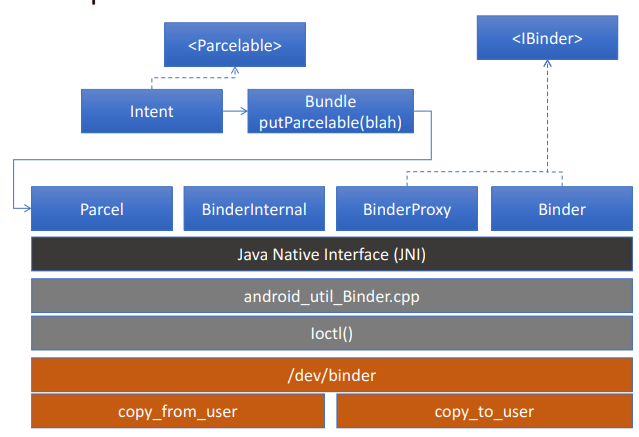
\includegraphics[scale=0.5]{binder_implem.png}
\end{center}

\newpage

\begin{description}
	\item[placeholder] \hfill \\
\end{description}
\end{document}
